\chapter{Microprocessors and Micro Controllers}\label{chap7}

Today we are living in the world of computers. Computers have invaded all sectors of society. We use computers at home, at offices, for our day to day activities. The brain of the computer is the CPU (Central Processing Unit), which is built using a micro processor or several microprocessors depending upon the complexity of the computing system. The microprocessor is a programmable logic device that can be used to do a variety of tasks ranging from a very simple to a very complicated one. Today we have embedded systems designed to perform a one and only one task. The brain of an embedded system is a micro controller. 

This chapter discusses the basics of microprocessors and micro controller. The architecture of 8085 microprocessor and 8051 micro controller has been discussed. Their applications are also discussed.

\section{Microprocessor}\label{sec7.1}

A microprocessor\index{Microprocessor} is a multipurpose, programmable logic device that reads binary instructions from a storage device called memory, accepts binary data as input and processes data according to those instructions and provides results as output.

Fig.~\ref{fig7.1} shows a typical programmable machine. It consists of three components.
\begin{itemize}
\item[(1)] Microprocessor

\item[(2)] Memory and

\item[(3)] Input\,/\,output (I\,/\,O) devices
\end{itemize}

These three components work together to perform a given task. They said to form a system. The physical components of this system are called hardware. A set of instructions written for the microprocessor to perform a task is called a program. A group of programs is called software.

\begin{figure}[H]
\centering
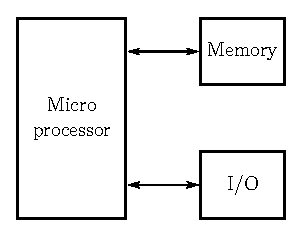
\includegraphics{chap7/fig7.1.eps}
\bigskip
\caption{Programmable Machine}\label{fig7.1}
\end{figure}

The system shown in Fig.~\ref{fig7.1} can be programmed to perform a task which can be a simple or a sophisticated one. Few examples of the task are~:
\begin{itemize}
\item turn traffic lights on and off

\item compute mathematical functions

\item playing video games

\item payroll, business accounts when used as CPU of a computer
\end{itemize}

\subsection{Word length of a microprocessor}\label{sec7.1.1}
\index{Microprocessor!word length of}

The microprocessor operates on binary digits, 0 and 1, also known as bits. Bit is an abbreviation for the term binary digit.

Each microprocessor recognises and processes a group of bits called the word. The microprocessors are classified according to their word length.
\begin{itemize}
\item A processor with an $8$-bit word is known as an $8$-bit microprocessor. 8085 is an $8$-bit microprocessor.

\item A processor with 16 bit word is known as a 16 bit microprocessor. 8086 is a 16 bit microprocessor.

\item 80386 is a 32 bit processor with a word length of 32 bits.
\end{itemize}

World length also indicates the number of bits that the processor can process at a time. For instance, a 16 bit processor can add two 16 bit binary numbers at a time. As the word length increases the processor becomes faster and more powerful.

\eject

\subsection{Grouping of bits}

Nibble~: A group of 4 bits.

\noindent
Byte~~~~~\!: A group of 8 bits.
\begin{itemize}
\itemsep=0pt
\item A byte has two nibbles.

\item A word of 16 bits has two bytes.

\item A word of 32 bits has 4 bytes.

\item A word of 64 bits has 8 bytes.
\end{itemize}
Generally the word length of a processor/computer is expressed in terms of bytes.

\section{Scale of Integration}\label{sec7.2}

Integration is the process of fabricating discrete logic gates on a semiconductor chip. Depending upon the number of gates fabricated on a chip, we have the following scales of integration.

\medskip
\heading{Small Scale Integration (SSI)}\index{Small Scale Integration}

It is the process of designing a few gates (10 gates) on a single chip.

\medskip
\heading{Medium Scale Integration (MSI)}\index{Medium Scale Integration}

It is the process of designing more than a hundred gates on a single chip.

\medskip
\heading{Large Scale Integration (LSI)}\index{Large Scale Integration}

It is the process of designing more than a thousand gates on a single chip.

\medskip
\heading{Very Large Scale Integration (VLSI)}\index{Very Large Scale Integration}

It is the process of designing ten thousand or more gates on a single chip.

Today we are in the era of VLSI technology.

\section{Microprocessor - Based System}\label{sec7.3}

The microprocessor is not complete by itself and has very limited memory on chip. Hence, for it to be of use, it must be interfaced with memory, input and output devices as shown in Fig.~\ref{fig7.2}.

The entire group of components is referred to as a system or micro computer system. Note that microprocessor is one component of micro computer and the micro computer is a complete computer similar to any other computer. The functions of components of a micro computer is explained below.
\begin{figure}[H]
\centering
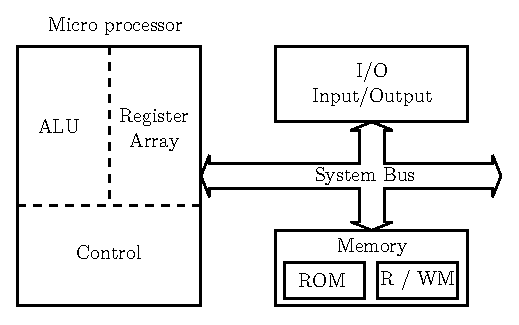
\includegraphics[scale=.92]{chap7/fig7.2.eps}
\caption{Microprocessor Based System}\label{fig7.2}
\end{figure}

\section{Microprocessor}\label{sec7.4}

The microprocessor is a semiconductor device consisting of electronic logic circuits manufactured by using either a large-scale integration (LSI) or very-large-scale integration (VLSI) technique. The microprocessor is capable of performing various computing functions and making decisions to change the sequence of program execution. The microprocessor can be divided into three segments\index{Microprocessor!segments} as shown in Fig.~\ref{fig7.2}.\\[-20pt]

\subsection{Arithmetic\,/\,Logic Unit (ALU)}\label{sec7.4.1}
\index{Arithmetic and Logic Unit}

The various computing functions on data are performed in the arithmetic\,/\,logic unit (ALU) of the microprocessor. The ALU performs
\begin{itemize}
\item Arithmetic operations such as addition and subtraction.

\item Logic operations such as AND, OR and EXOR operations.
\end{itemize}
The results of arithmetic and logic operations are stored in registers or memory.\\[-20pt]

\subsection{Register Array}\label{sec7.4.2}
\index{Register Array}

Register array consists of various registers. These registers are primarily used to store data temporarily during the execution of a program. The user can access some of the registers through program instructions.\\[-20pt]

\subsection{Control Unit}\label{sec7.4.3}
\index{Control Unit}

The necessary timing and control signals to all the operations in the micro computer is provided by the control unit. The flow of data between the microprocessor and memory and I\,/\,O devices is controlled by the control unit.

\vfill\eject

\subsection{Memory}\label{sec7.4.4}
\index{Memory}

Memory stores binary information and provides that information to the processor when ever necessary. The binary information comprises of instructions and data. To execute programs, the microprocessor reads instructions and data from memory and performs the computing operations in ALU section. Results are either stored in memory for future use or sent to the output section for display.

The memory has two sections.
\begin{itemize}
\item[(1)] Read-only memory (ROM).

\item[(2)] Read write memory (R\,/\,WM) or Random-Access memory (RAM).
\end{itemize}

The ROM is used to store programs that do not need alterations. Programs stored in the ROM can only be read. They cannot be altered.

The Read\,/\,Write memory (R\,/\,WM) also known as user memory is used to store user program and data. The information stored in this memory can be easily read and altered.

\subsection{I\,/\,O (Input\,/\,Output)}\label{sec7.4.5}

It interfaces the system with the outside world. I\,/\,O includes two types of devices.
\begin{itemize}
\item[(1)] Input Device.\qquad\quad (2)~ Output Device.
\end{itemize}
I\,/\,O devices are also called as peripherals.\index{Peripherals}

The input device transfers data and instruction in binary form from the outside world to the microprocessor. Examples of input devices are keyboard, mouse, switches etc.

The output devices transfer data from the microprocessor to the outside world. Examples of output devices are monitor, printer, cathode ray tube (CRT) light emitting diodes (LEDs) etc.

\subsection{System Bus}\label{sec7.4.6}

The system bus\index{System bus} is a communication path between the microprocessor and peripherals. Bus is nothing but a group of wires to carry bits\,: each wire carrying one bit.

\section{Working of Microprocessor}\label{sec7.5}
\index{Microprocessor!working of}

Now let us understand how the microprocessor executes the programs.

The program to perform a specified task is sequentially stored in the R\,/\,W memory. The data to be used by the programs also stored in the R\,/\,W memory. The program and data are in the binary form. When the execute command is given the following sequence of operations takes place.
\begin{itemize}
\itemsep=0pt
\item The microprocessor fetches the first instruction.

\item It decodes the instruction and

\item Executes that instruction.
\end{itemize}

The fetch, decode and execute sequence is continued until the microprocessor comes across an instruction to stop.


During the entire process the microprocessor
\begin{itemize}
\itemsep=0pt
\item Uses the system bus to fetch the binary instructions and data from the memory.

\item Uses registers from the register section to store data temporarily. 

\item Performs the computing function in the ALU section.

\item Sends out the result in binary, using the same bus lines to the output device.
\end{itemize}

\section{Computer Languages}\label{sec7.6}
\index{Computer Languages}

Language is a medium of communication through which the programmer or the user can communicate with the microprocessor or a computer. We have the following classification of computer languages.

\medskip
\heading{1. Machine language}
\index{Machine language}

Each microprocessor has its own set of instructions based on its architecture. The instructions are in the binary form. The binary language used by the programmes to communicate with the microprocessor is called the machine language.

For Example~:

0011 1100 is an instruction in 8085 microprocessor that increments the number in register A of 8085 by one.

\medskip
\heading{2. Assembly language}
\index{Assembly language}

Since it is difficult for most people to write programs in sets of 0's and 1's, computer manufacturers have devised english like words to represent the binary instructions of a microprocessor. Programs written using these english like words is called Assembly Language Programs. The english like words used to represent the binary instructions are called mnemonics.

For Example~:

INR A\qquad is a mnemonic in 8085 microprocessor that increments the number in register A by one.

Machine language and Assembly language are called low level languages since these languages are specific to a microprocessor.

\medskip
\heading{3. High level language}
\index{High level language}

\smallskip

Since Assembly language is specific to a given machine, programs written in assembly language for one machine can not be run on another machine. To overcome this problem, general purpose programs have been devised. These machine independent languages are called high level languages. Some examples of high level languages are FORTRAN, BASIC, C, C++ etc.

\section{Combinations with \boldmath$n$-bit binary word}\label{sec7.7}

With 2 binary bits, we can form $2^{2}=4$ combinations of two bits each. They are 00, 01, 10 and 11. In general with $n$ binary bits, $2^{n}$ combinations of $n$ bits each can be formed. Table~\ref{tab7.1} gives the possibles combinations of binary word for $n$ ranging from 8 to 16.

\smallskip
\begin{table}[h]
\centering
\caption{Possible combinations of binary word}\label{tab7.1}
\renewcommand{\arraystretch}{1.05}
\tabcolsep=10pt
\begin{tabular}{|c|c|}
\hline
{\boldmath$n$} & {\bf Possible Combinations}\\
\hline
8 & 256\\
9 & 512\\
10 & 1024 (1K)\\
11 & 2048 (2K)\\
12 & 4096 (4K)\\
13 & 8192 (8K)\\
14 & 16384 (16K)\\
15 & 32768 (32K)\\
16 & 65536 (64K)\\
\hline
\end{tabular}
\end{table}

\section{The 8085 Microprocessor}\label{sec7.8}
\index{8085 Microprocessor}

The 8085\index{Microprocessor!8085} is an 8 bit general purpose microprocessor capable of addressing 64K memory locations. The device has 40 pins and requires a +5V single power supply. It can operate with a 3-MHz single-phase clock.

Fig.~\ref{fig7.3} shows the logic pin out of the 8085 microprocessor. All signals can be classified into six groups.
\begin{itemize}
\itemsep=0pt
\item[(1)] Address bus

\item[(2)] Data bus

\item[(3)] Control and status signals

\item[(4)] Power supply and frequency signals

\item[(5)] Externally initiated signals and

\item[(6)] Serial I\,/\,O ports
\end{itemize}
\vskip -.5cm
\begin{figure}[H]
\centering
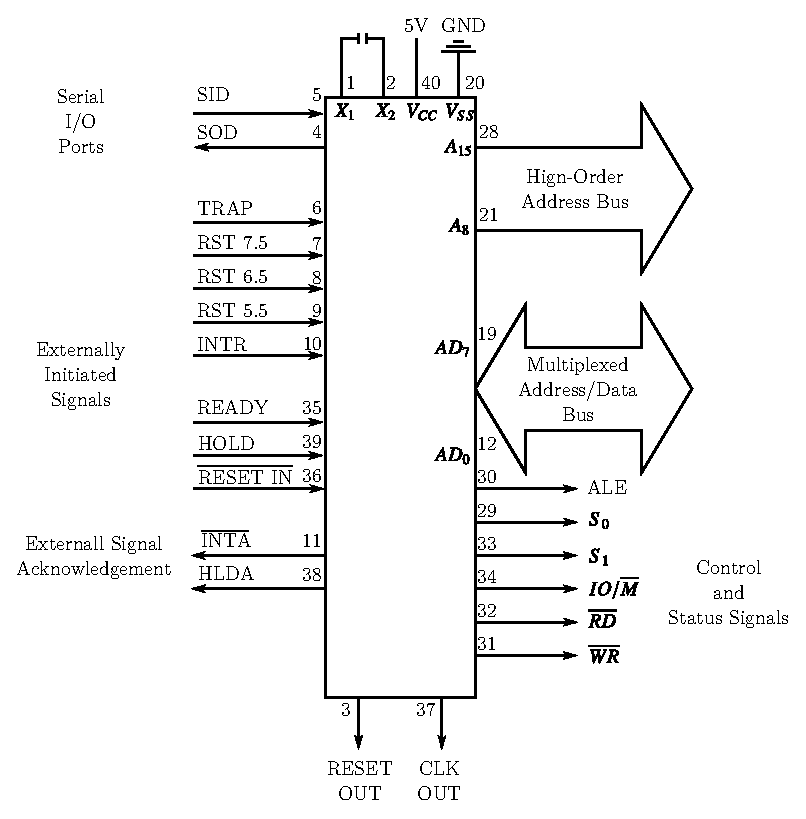
\includegraphics{chap7/fig7.3.eps}
\caption{Logic Pin Out of 8085 (Courtesy : Intel)}\label{fig7.3}
\end{figure}
The brief functioning of these signals is covered in the next section.

\subsection{Features of 8085 microprocessor}\label{sec7.8.1}
\index{Microprocessor!features of}\index{8085 Microprocessor!features of}

The 8085 microprocessor has the following features.
\begin{enumerate}
\renewcommand{\labelenumi}{$\bullet$}
\itemsep=7pt
\item It is a 40 pin IC manufactured using VLSI technology.

\item It operates with a single power supply of +5V (dc).

\item It operates at a clock frequency of 3\,MHz. A crystal having a frequency of 6\,MHz should be connected between the pins $X_{1}$ and $X_{2}$ to operate the system at 3\,MHz, since the frequency is internally divided by two.

\item It is an 8 bit processor meaning that it can process 8 bits at a time.

\item It has 8 bit data bus~: $A_{D_{7}}-A_{D_{0}}$.

\item It has 16 bit address bus~: $A_{15}-A_{8}\,A_{D_{7}}-A_{D_{0}}$
\begin{itemize}
\item $A_{15}-A_{8}$ is called high order address bus which carries the higher 8 bits of the 16 bit address.

\item $A_{D_{7}}-A_{D_{0}}$ is called the low order address bus which carries the lower 8 bits of 16 bit address.

\item With 16 bit address bus, 8085 can address 64K memory locations, each of 8 bit wide.
\end{itemize}

\item To reduce the pin count, the data bus $A_{D_{7}}-A_{D_{0}}$ is also used as the low order address bus, since address and data are not sent at the same time. This technique is called multiplexing and $A_{D_{7}}-A_{D_{0}}$ is called multiplexed address-data bus. While using $A_{D_{7}}-A_{D_{0}}$ as data bus, it should be demultiplexed from the address bus. ALE (address latch enable) signal is used for demultiplexing the data bus.

\item It uses $A_{D_{7}}-A_{D_{0}}$ to address I\,/\,O devices. Hence 256($2^8$) input and 256 output devices can be addressed.

\item It supports 74 groups of instructions which covers almost all logical and arithmetic operations.

\item The ALU of 8085 can performs
\begin{itemize}
\item[(a)] 8 bit binary addition with and with out carry.

\item[(b)] 16 bit binary addition.

\eject

\item[(c)] 2 digit $BCD$ addition.

\item[(d)] 8 bit binary subtraction with and with out borrow.

\item[(e)] 8 bit logical operations such as AND, OR, EX-OR, complement (NOT) and shift operations.
\end{itemize}

\item It has five interrupt signals~:
\begin{center}
TRAP, \ RST\;7.5, \ RST\;6.5, \ RST\;5.5 \ and \ INTR.
\end{center}
Interrupts are used to interrupt a program execution.

\item It has two serial I\,/\,O pins~:

SID (Serial input data) and SOD (Serial output data) for serial transmission of data.

\item It has two control signals $\overline{\rm RD}$ and $\overline{WR}$ and three status signals IO/$\overline{\rm M}$, $S_{1}$ and $S_{0}$ to identify whether the operation is fetch, read or write.

\item It is capable of performing huge data transfer at high speed using DMA (Direct memory access) technique.

\item By interfacing with external memory and I\,/\,O devices an 8085 based micro computer system can be built.
\end{enumerate}

\section{Architecture of 8085 microprocessor}\label{sec7.9}
\index{Microprocessor!architecture of}\index{8085 Microprocessor!architecture of}

The microprocessor is a programmable logic device, designed with registers, flip-flops and timing circuits. The logic design of the microprocessor is called its architecture.

Fig.~\ref{fig7.4} shows the architecture of 8085 microprocessor. It is also called the functional block diagram.

\vskip .1cm
It consists of the following functional blocks.
\begin{enumerate}
\renewcommand{\labelenumi}{$\bullet$}
\item Register array

\item Arithmetic\,/\,Logic Unit (ALU)

\item Timing and Control Unit

\item Instruction Register and Decoder
\end{enumerate}
\begin{landscape}
\begin{figure}[H]
\centering
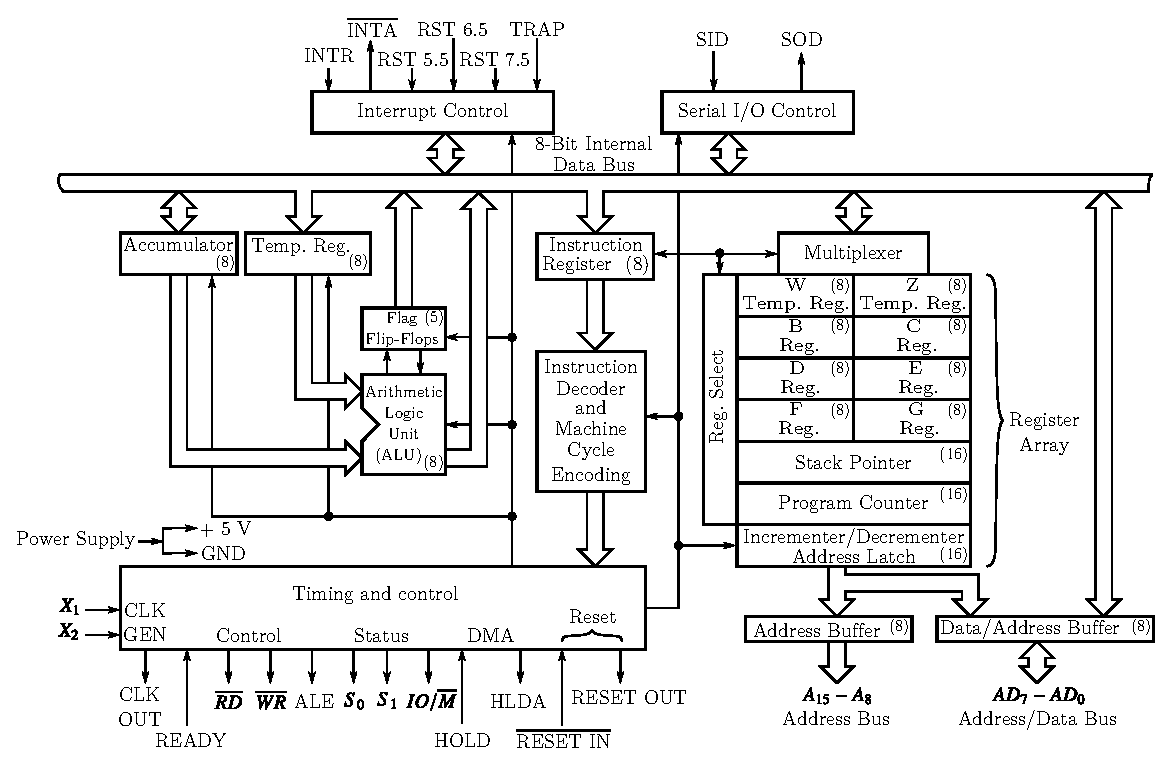
\includegraphics[scale=.97]{chap7/fig7.4.eps}
\medskip
\caption{Functional block diagram of 8085 (Courtesy : Intel)}\label{fig7.4}
\end{figure}
\end{landscape}

\subsection*{Register Array}
\index{Microprocessor!register array}\index{8085 Microprocessor!register array}

Register array consists of the following registers.
\begin{itemize}
\itemsep=2pt
\item[(a)] General purpose registers

\item[(b)] Special purpose registers

\item[(c)] Temporary registers

\item[(d)] Sixteen bit registers
\end{itemize}

\smallskip
\heading{General purpose registers}
\index{Microprocessor!general purpose registers}\index{8085 Microprocessor!general purpose registers}

The 8085 has six general purpose registers to store 8 bit data during program execution. These registers are identified as B, C, D, E, H and L. They can be combined as register pairs - BC, DE and HL - to perform some 16 bit operations. These registers are also called programmable registers since they are accessible to the user through instructions.

\smallskip
\heading{Special purpose registers}
\index{Microprocessor!special purpose registers}\index{8085 Microprocessor!special purpose registers}

The special purpose registers are the accumulator and Flag register.

\smallskip
\heading{Accumulator}
\index{Microprocessor!accumulator}\index{8085 Microprocessor!accumulator}

Accumulator\index{Accumulator} is also called the register A. It is an 8 bit register and is a part of ALU. This register is used while performing arithmetic and logical operations. The result of an operation is stored in the accumulator.

\smallskip
\heading{Flag register}
\index{Microprocessor!flag register}\index{8085 Microprocessor!flag register}

Flag register\index{Flag register} is also a part of ALU and has five flip-flops. These flip-flops are set or reset according to data conditions in the accumulator and other registers. Fig.~\ref{fig7.5} shows the flag register.
\begin{figure}[H]
\centering
\caption{Flag register}\label{fig7.5}
\renewcommand{\arraystretch}{1.2}
\begin{tabular}{|c|c|c|c|c|c|c|c|c}
\multicolumn{1}{c}{$D_{7}$} & \multicolumn{1}{c}{$D_{6}$} & \multicolumn{1}{c}{$D_{5}$} & \multicolumn{1}{c}{$D_{4}$} & \multicolumn{1}{c}{$D_{3}$} & \multicolumn{1}{c}{$D_{2}$} & \multicolumn{1}{c}{$D_{1}$} & \multicolumn{1}{c}{$D_{0}$} & \multicolumn{1}{c}{}\\
\cline{1-8}
S & Z & X & AC & X & P & X & CY &~~~ X : Not used\\
\cline{1-8}
\end{tabular}
\end{figure}

\noindent
{\bf S - Sign Flag~:}\index{Sign Flag} After the execution of an arithmetic or logical operation, the sign flag is set, if bit $D_{7}$ of the result is 1. In a given byte if $D_{7}$ is 1, the number is viewed as a negative number. If $D_{7}$ is $0$ the number is considered as a positive number.

\medskip
\noindent
{\bf Z - Zero Flag~:}\index{Zero Flag} If the result of an arithmetic or logical operation is zero, the zero flag\index{Flag} is set. If the result is non zero, the zero flag is reset.

\eject

\medskip
\heading{AC-Auxiliary Carry Flag~:}
\index{Auxiliary Carry Flag}

In an arithmetic operation, when a carry is generated by bit $D_{3}$ and passed onto bit $D_{4}$ (lower nibble to higher nibble), the AC flag is set. This flag is used only internally for BCD (binary-coded decimal) operations and not available to the programmer.

\medskip
\noindent
{\bf P - Parity Flag~:}\index{Parity Flag} After an arithmetic or logical operation if the result has an even number of 1's, the flag is set. If it has an odd number of 1's, the flag is reset.
\begin{description}
\item[Example~:] 0011 0011 has even number of 1's.

\qquad~ 0100 1111 has odd number of 1's.
\end{description}

\noindent
{\bf CY - Carry Flag~:}\index{Carry Flag} If an arithmetic operation results in a carry, the carry flag is set. Otherwise reset. The carry flag also serves as a borrow flag for subtraction.

Observe from Fig.~\ref{fig7.5} that, bits $D_{5}$, $D_{3}$ and $D_{1}$ of flag register are unused.

\medskip
\heading{Temporary Registers}
\index{Microprocessor!temporary registers}\index{8085 Microprocessor!temporary registers}

There are two types of temporary registers.
\begin{itemize}
\item[$\bullet$] Temporary data register.

\item[$\bullet$] $W$ and $Z$ registers.
\end{itemize}

Temporary data register is an 8 bit register which is used by the ALU during arithmetic and logical operations. For example, during the addition of two data bytes, one data byte must be in the accumulator. The other data byte which is stored in other register or memory is transferred to the temporary register by the microprocessor before addition and the result is stored in the accumulator.

$W$ and $Z$ registers are also 8 bits registers and are used to hold 8 bit data during the execution of some instructions. These registers are not available to the programmer.

\medskip
\heading{Sixteen bit registers}

There are two 16 bit registers namely programs counter (PC) and stack pointer (SP).

\medskip
\heading{Program counter (PC)}\index{Program counter}

This is a 16-bit register which is a memory pointer. 
The program counter\index{Microprocessor!program counter}\index{8085 Microprocessor!program counter} holds the address of the memory location from which the next instruction byte is to be fetched.

\medskip
\heading{Stack pointer (SP)}
\index{Stack pointer}

It is also a 16-bit register used as a memory pointer. It points to a memory location in R\,/\,W memory called stack. Stack is a portion of the RAM, set aside for the temporary storage of register contents. The beginning of the stack is defined by loading a 16-bit address in the stack pointer register.

\subsection*{Arithmetic and Logic Unit (ALU)}

The ALU performs arithmetic and logical operations on eight bit data. The ALU performs arithmetic operations such as addition and subtraction. It also performs logical operations such as complement, AND, OR and EX-OR, as well as rotate and clear. It stores the result in accumulator and sets or resets the flags according to the result of the operation.

\medskip
\heading{Timing and Control Unit}
\index{Timing and Control Unit}

This unit synchronizes all the microprocessor operations with the clock and generates the control signals necessary for communication between the microprocessor and peripherals.

\medskip
\heading{Instruction Register and Decoder}
\index{Instruction register}\index{Decoder}

The instruction register and the decoder are part of the ALU. The instruction fetched from the memory is first loaded in the instruction register. The decoder decodes the instruction and establishes the sequence of events to follow. Instruction register is not accessible through any instruction (not programmable).

\section{Applications of Microprocessor}\label{sec7.10}
\index{Microprocessor!applications of}

Microprocessors are used for wide range of applications. These applications can be broadly classified into two groups~: general purpose application and special purpose application.

\medskip
\heading{General purpose application}
\begin{enumerate}
\renewcommand{\labelenumi}{$\surd$}
\item Single board micro computers

\item Personal computers

\item Super minis and CAD.
\end{enumerate}

\heading{Special purpose application}

\begin{enumerate}
\renewcommand{\labelenumi}{\boldmath$\bullet$}
\item {\bf Instrumentation}
\begin{itemize}
\itemsep=4pt
\item[$\surd$] Controllers in various instruments.

\item[$\surd$] Medical instruments to measure blood pressure, temperature, heart rate etc.
\end{itemize}

\item {\bf Control}
\begin{itemize}
\itemsep=4pt
\item[$\surd$] Home appliances such as microwave oven, washing machine.

\item[$\surd$] In industry for controlling various process parameters such as speed, temperature, moisture and pressure.
\end{itemize}

\item {\bf Communication}
\begin{itemize}
\itemsep=6pt
\item[$\surd$] Digital telephone sets

\item[$\surd$] Modems

\item[$\surd$] Railway reservation

\item[$\surd$] Air ticket reservation

\item[$\surd$] Satellite communication

\item[$\surd$] Mobile phones

\item[$\surd$] Televisions
\end{itemize}

\medskip
\item {\bf Office Automation and Publication}
\begin{itemize}
\itemsep=6pt
\item[$\surd$] Word processing

\item[$\surd$] Spread sheet operations

\item[$\surd$] Storage and retrieval of huge information

\item[$\surd$] Automatic photo copies

\item[$\surd$] Laser printers
\end{itemize}
\end{enumerate}

\section{Micro Controller}\label{sec7.11}
\index{Micro Controller}

The micro controller can be viewed as computer on a single chip. This essentially means that the CPU, RAM, ROM and some other devices like timers, I/O ports etc are all located on the same chip as shown in Fig.~\ref{fig7.6}.
\begin{figure}[H]
\centering
\caption{Micro controller}\label{fig7.6}
\tabcolsep=10pt
\renewcommand{\arraystretch}{2}
\begin{tabular}{|c|c|c|}
\hline
CPU & RAM & ROM\\
\hline 
I\,/\,O & Timer & Serial COM port\\
\hline
\end{tabular}
\end{figure}

\newpage

\heading{Need for micro controller}

\smallskip

To build a minimum system using microprocessor the following external devices must be interfaced with the microprocessor.
\begin{itemize}
\item RAM and ROM, since the microprocessor has very limited memory on chip.

\item Programmable peripheral interface (PPI) since it has no inbuilt ports.

\item Other peripherals such as timers, ADC, DAC etc.,  

This makes the system very expensive for many of the applications such as Intercom, Cellular Phones, Camera, Security Systems, Washing Machines etc.
\end{itemize}
This led to the evolution of micro controllers.

\section{The 8051 Micro Controller}\label{sec7.12}
\index{8051 Micro Controller}

8051\index{Micro Controller!8051} is an 8 bit micro controller manufactured using VLSI technology. It was introduced by Intel Corporation in the year 1980. Fig.~\ref{fig7.7} shows the block diagram of 8051 micro controller.
\begin{figure}[H]
\centering
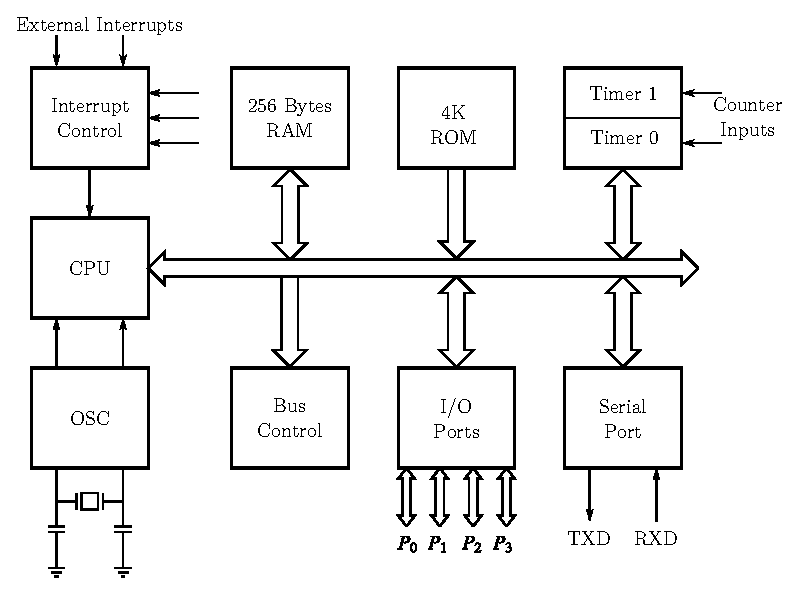
\includegraphics[scale=.9]{chap7/fig7.7.eps}
\medskip
\caption{Block diagram of 8051}\label{fig7.7}
\end{figure}

\section{The Salient Features of 8051 are as follows}\label{sec7.13}

The Salient features of\index{Micro Controller!features of}\index{8051 Micro Controller!features of} 8051 are as follows.
\begin{itemize}
\itemsep=0pt
\item $8$-bit CPU with two registers: {\em Accumulator} (register A) and register B. Accumulator is used in most arithmetic and logic operations. Register B is used for integer multiplication and division.

\item A $16$-bit register called {\em Program Counter} (PC). It holds the address of the location of the next instruction to be executed.

\item A $16$-bit {\em Data Pointer} (DPTR) register. It is used to access external memory.

\item An $8$-bit {\em Program Status Word} (PSW) register. It indicates certain conditions like status of carry, parity, sign etc, after execution of some instructions.

\item {\em Internal RAM} of 256 bytes divided as
\begin{itemize}
\itemsep=-.5pt
\item[$\surd$] Four register banks of 8 registers each (Total 32 bytes).

\item[$\surd$] Sixteen bytes, which are bit addressable. The individual bits of these bytes can be altered.

\item[$\surd$] Eighty bytes of general RAM memory.

\item[$\surd$] 128 Special function registers each of 8 bit wide.
\end{itemize}

\item 4K Internal ROM to store program code.

\item Four 8-bit {\em Ports,} P0 to P3. A port pin is a pin, where data can be transmitted to (output) or read (input) from an external device.

\item Two sixteen bit timers, {\em Timer $0$ and Timer $1$.} The timers can be used in Timer mode when counting internal clock pulses and in counter mode when counting external pulses.

\item Full duplex {\em serial data transmitter\,/\,receiver} register, SBUF. This holds the byte to be transmitted or the received byte, when serial communication is used.

\item Two external interrupts and three internal interrupts. Interrupts are events which interrupt the normal sequence of execution of instructions.

\item {\em Control registers~:} TCON, TMOD, SCON, PCON, IP and IE which control the operations of the timers, serial port and interrupts.

\item {\em Oscillator and clock circuits} : operates at a clock frequency of 12\,MHz.
\end{itemize}

\section{Architecture of 8051}\label{sec7.14}
\index{Micro Controller!architecture of}\index{8051 Micro Controller!architecture of}

Fig.~\ref{fig7.8} shows the functional block of the internal operations of an 8051 micro controller which is also called its architecture. The architecture consists of the following blocks.
\begin{figure}[H]
\centering
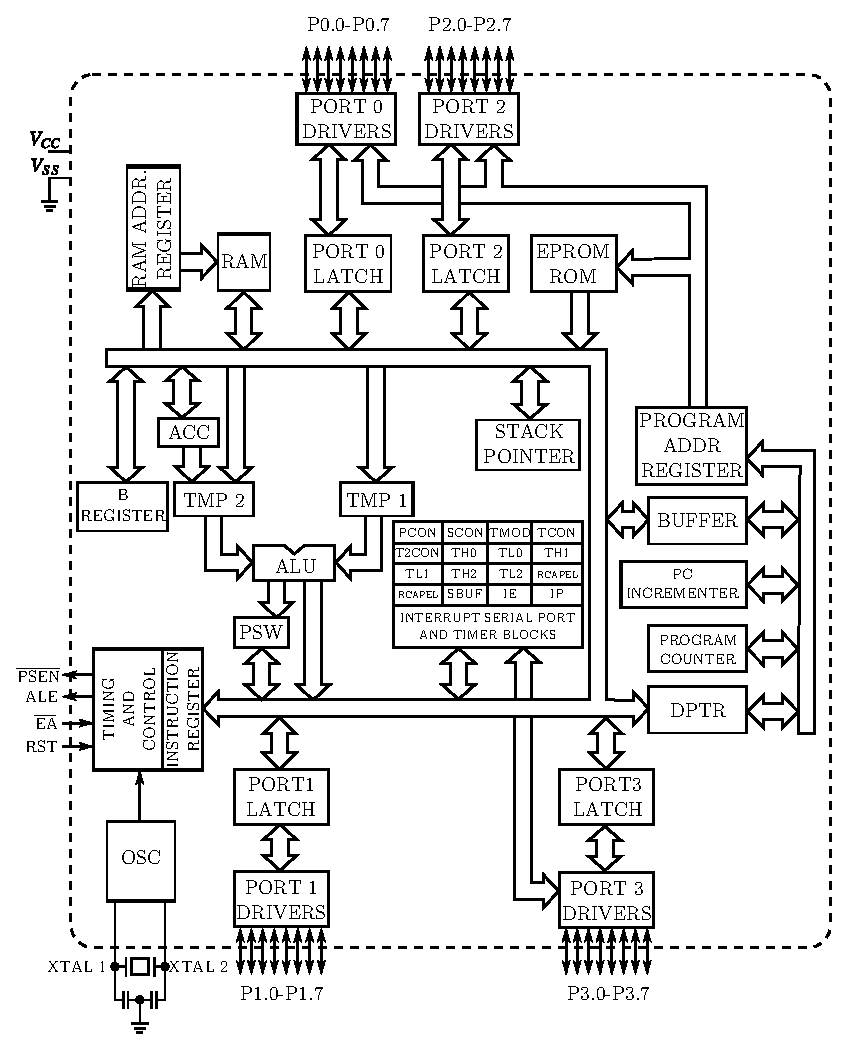
\includegraphics{chap7/fig7.8.eps}
\caption{Functional block diagram of 8051 (Courtesy : Intel)}\label{fig7.8}
\end{figure}
\begin{itemize}
\itemsep=2pt
\item[$\bullet$] Processor

\item[$\bullet$] Memory

\item[$\bullet$] Digital I\,/\,O port and peripherals
\end{itemize}

\subsection*{Processor (CPU)}
\index{Micro Controller!processor}\index{8051 Micro Controller!processor}

The processor includes the following units.
\begin{itemize}
\itemsep=2pt
\item Arithmetic and logic unit (ALU)

\item Intruction decoder and timing generation unit and 

\item Registers
\end{itemize}

\medskip
\heading{Arithmetic and logic unit (ALU)}
\index{Micro Controller!arithmetic and logic unit}\index{8051 Micro Controller!arithmetic and logic unit}

\vskip .1cm
The ALU performs the arithmetic and logical operations. In arithmetic and logical operations, one of the operand is in $A$ register. The results of arithmetic/logical operations are stored in $A$ register and the flags of program status word are affected according to the results.


\medskip
\heading{Instruction Decoder and Control}
\index{Micro Controller!instruction decoder}\index{8051 Micro Controller!instruction decoder}

\vskip .1cm
When an instruction is fetched from program memory, it is loaded in the instruction register. The decoder decodes the instruction and establishes the sequence of events to follow.

The timing generation and control unit synchronises all the micro controller operations with the clock and generates control signals necessary for communication between the processor and peripherals.

\medskip
\heading{CPU Registers}
\index{Micro Controller!CPU registers}\index{8051 Micro Controller!CPU registers}

\vskip .1cm
The CPU contains the following registers.
\begin{itemize}
\itemsep=0pt
\item[$\surd$] A register (Accumulator) 

\item[$\surd$] B Register 

\item[$\surd$] Program status word register

\item[$\surd$] Stack pointer

\item[$\surd$] Data pointer

\item[$\surd$] Program counter
\end{itemize}

\eject

\heading{A Register}

It is an 8 bit register and is also called the accumulator. It is used in all arithmetic and logical operations.
\begin{itemize}
\itemsep=0pt
\item In multiplication operation the lower type of the result is stored in accumulator.

\item In division operation, it holds the 8 bit dividend. After division operation the quotient is stored in the accumulator.

\item It is also used in indexed addressing mode to access information from the program memory.

\item It is a bit addressable register. 
\end{itemize}

\heading{B Register}

It is an 8 bit register.
\begin{itemize}
\itemsep=0pt
\item In multiplication operation, one of the 8 bit operand is stored in register B. After the operation the higher byte of the result is stored in B register.

\item In division operation, it holds 8 bit divisor. After the operation the remainder is stored in B register.

\item It can also be used as an 8 bit general purpose register and it is bit addressable.
\end{itemize}

\heading{Program status word register}

\smallskip
It is an 8 bit register in which 7 bits are used as flags to indicate the status of an arithmetic\,/\,logical operation. It is shown in Fig.~\ref{fig7.9}.
\begin{figure}[H]
\centering
\caption{Processor status word register}\label{fig7.9}
\renewcommand{\arraystretch}{1.2}
\begin{tabular}{|c|c|c|c|c|c|c|c|}
\hline
CY & AC & F0 & RS1 & RS0 & OV & \ldots & P\\
\hline
\multicolumn{1}{c}{Bit 7} & \multicolumn{5}{c}{} & \multicolumn{1}{c}{Bit 1} & \multicolumn{1}{c}{Bit 0}
\end{tabular}
\end{figure}

\heading{CY - Carry\,/\,borrow bit}

\begin{itemize}
\item CY bit is set when the addition of two 8 bit operands results in a carry. Otherwise it is reset.

\item CY bit is also set if the borrow occurs during the subtraction of two 8 bit operands. Otherwise it is reset.
\end{itemize}

\heading{AC - Auxiliary Carry\,/\,borrow bit}

AC bit is set when there is a carry from lower nibble to higher nibble. Otherwise it is cleared.

\medskip
\heading{F0 - Flag 0}\index{Micro Controller!flag}\index{8051 Micro Controller!flag}

It is available to the user for general purpose.

\heading{RS1 : RS0~ register bank select bits}

\smallskip
These bits are used to select the register bank of 8051. The selection logic is as follows.
\begin{center}
\renewcommand{\arraystretch}{1.2}
\begin{tabular}{|c|c|}
\hline
RS1\quad RS0 & Register Bank selected\\
\hline
0~ 0 & Bank 0\\
0~ 1 & Bank 1\\
1~ 0 & Bank 2\\
1~ 1 & Bank 3\\
\hline
\end{tabular}
\end{center}
Each bank contains eight registers each of 8 bits.

\medskip
\heading{OV - Overflow}

\smallskip
This flag is used to detect errors in signed arithmetic operations. OV is set;
\begin{itemize}
\item If there is a carry from $D_{6}$ to $D_{7}$ but no carry from $D_{7}$ or

\item If there is a carry from $D_{7}$ but no carry from $D_{6}$ to $D_{7}$.
\end{itemize}
{\bf Bit 1~:} This flag bit is not defined.

\medskip
\heading{P - Parity Flag}

\smallskip
This flag is set if the result of an arithmetic or logical operation has even number of 1's. Otherwise it is reset.

\medskip
\heading{Stack Pointer}

\smallskip
It is an 8 bit register. It contains the address of the top of the stack. Stack is a portion of the on chip RAM, set aside for the temporary storage of register contents.

\medskip
\heading{Data Pointer (DPTR)}

\smallskip
It consists of two 8 bit registers~:

DPH - High byte

DPL - low byte
\begin{itemize}
\item It is intended to hold a 16 bit address.

\item It is used to furnish address information for internal and external program memory and for external data memory.
\end{itemize}

\heading{Program Counter (PC)}\index{Micro Controller!program counter}\index{8051 Micro Controller!program counter}

\smallskip
It is a 16 bit register. It holds the address of the next instruction to be executed.

\eject

\heading{Memory}
\index{Micro Controller!memory}\index{8051 Micro Controller!memory}

\smallskip
The 8051 has 4k bytes on-chip data RAM. The program memory is used to hold the start up program that will be executed when the 8051 is powered up.

The organisation of on-chip data RAM as shown in Fig.~\ref{fig7.10}.
\begin{figure}[H]
\centering
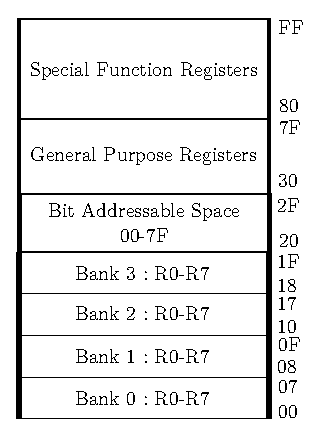
\includegraphics{chap7/fig7.9.eps}
\caption{Internal RAM organisation}\label{fig7.10}
\end{figure}

\medskip
\heading{Register Banks (00H - IFH)}
\index{Micro Controller!register banks}\index{8051 Micro Controller!register banks}

\smallskip
There are four register banks each bank consisting of 8 bit general purpose registers, $R_{0}$-$R_{7}$. The register banks are selected using register bank select bits $RS_{1}:RS_{0}$.

\medskip
\heading{Bit Addressable RAM (20H - 2FH)}

\smallskip
This area of RAM contains 16 registers each of 8 bits. Each bit of these 16 registers can be set or cleared.

\medskip
\heading{General purpose RAM (30H - 7FH)}

\smallskip
This area of RAM contains 80 bytes of RAM which are available for general purpose data storage.

\medskip
\heading{Special Function Registers (SFR : 80H - FFH)}

\smallskip
SFR registers contain
\begin{itemize}
\item input and output ports\qquad $\bullet$~ control register for interrupts

\item timers\hspace{3.1cm} $\bullet$~ serial ports etc.
\end{itemize}

\heading{Digital I\,/\,O ports and peripherals}

\smallskip
It contains four 8 bit parallel ports named as port 0, port 1, port 2 and port 3.
\begin{itemize}
\item Each bit of the port can be configured as an input to send data or an output to receive data.

\item Port 0 is also used as the low order address and data lines ($A_{D_7}$-$A_{D_0}$).

\item Port 2 is also used as high order address lines.

\item Port 3 is also used by timers, serial port, external interrupt and for sending control signals $\overline{\rm RD}$ and $\overline{\rm WR}$.
\end{itemize}

\section{Applications of Micro Controllers}\label{sec7.15}
\index{Microprocessor!applications of}

Micro Controllers are extensively used in embedded systems. A system which is designed to perform only one task is called an embedded system. In an embedded system the application software intended to perform only one application is burnt into the ROM.

Following are some applications, where uses micro controllers are being used.

\smallskip
\heading{Home Appliances}
\begin{center}
\begin{tabular}{l@{\;\,}l@{\qquad}l@{\;\,}l@{\qquad}l@{\;\,}l}
$\bullet$ & Inter com & $\bullet$ & VCR & $\bullet$ & Cellular phones\\[4pt]
$\bullet$ & Video games &$\bullet$ & Camera & $\bullet$ & Fax machines\\[4pt]
$\bullet$ & Television & $\bullet$ & Security systems etc.
\end{tabular}
\end{center}

\heading{Office}
\begin{center}
\begin{tabular}{l@{\;\,}l@{\qquad}l@{\;\,}l@{\qquad}l@{\;\,}l}
$\bullet$ & Telephones & $\bullet$ & Computers & $\bullet$ & Security systems\\[4pt]
$\bullet$ & Laser Printers & $\bullet$ & Computers & $\bullet$ &
Air conditioners\\[4pt]
$\bullet$ & Heaters etc.
\end{tabular}
\end{center}

\heading{Others}
\begin{center}
\begin{tabular}{l@{\;\,}l@{\qquad}l@{\;\,}l@{\qquad}l@{\;\,}l}
$\bullet$ &  Instrumentation & $\bullet$ & Space craft\\[4pt]
$\bullet$ &  Smart cards & $\bullet$ & Entertainment etc.
\end{tabular}
\end{center}

\eject

\section{Differences between Microprocessor and Micro Controller}\label{sec7.16}

Table~\ref{tab7.2} summarizes the differences between microprocessor and micro controller.
{\fontsize{10pt}{12pt}\selectfont
\begin{longtable}{|p{6.8cm}|p{6.8cm}|}
\caption{Differences between microprocessor and micro controller}\label{tab7.2}\\
\hline
\multicolumn{1}{|c|}{\bf Microprocessor} & \multicolumn{1}{c|}{\bf Micro Controller}\\
\hline
&\\[-2pt]
\multicolumn{1}{|c|}{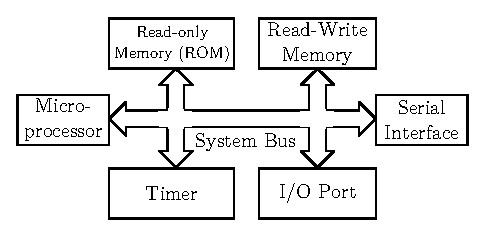
\includegraphics[scale=.87]{chap7/tab7.1a.eps}} & \multicolumn{1}{c|}{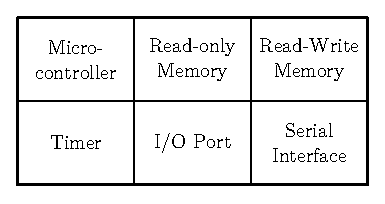
\includegraphics[scale=.87]{chap7/tab7.1b.eps}}\\[4pt]
\hline
Microprocessor is the heart of Computer system. & Micro Controller is the heart of embedded system.\\
\hline
It is just a processor. Memory and I\,/\,O components have to be connected externally. & Micro controller has external processor along with internal memory and I\,/\,O components.\\
\hline
Since memory and I\,/\,O units are to be connected externally, the circuit becomes large. & Since memory and I/O are present internally, the circuit is small.\\
\hline
Cannot be used in compact systems and hence inefficient. & Can be used in compact systems and hence it is an efficient technique.\\
\hline
Cost of the entire system is high. & Cost of the entire system is low.\\
\hline
Due to external components, the entire power consumption is high. Hence it is not suitable to use with devices running on stored power like batteries. & Since external components are less, total power consumption is less and can be used with devices running on stored power like batteries.\\
\hline
Most of the microprocessors do not have power saving features. & Most of the micro controllers have power saving modes like idle mode and power saving mode. This helps to reduce power consumption even further.\\
\hline
Since memory and I\,/\,O components are all external, each instruction will need external operation, hence it is relatively slower. & Since components are internal, most of the operations are internal instruction, hence speed is fast.\\
\hline
Microprocessor has less number of registers, hence more operations are memory based. & Micro controller has more number of registers, hence the programs are easier to write.\\
\hline
Microprocessors are based on von Neumann model/architecture where program and data are stored in same memory module. & Micro controllers are based on Harvard architecture where program memory and data memory are separate.\\
\hline
\end{longtable}}
